%% LyX 1.6.1 created this file.  For more info, see http://www.lyx.org/.
%% Do not edit unless you really know what you are doing.
\documentclass[english]{article}
\usepackage[T1]{fontenc}
\usepackage[latin9]{inputenc}
\usepackage{geometry}
\geometry{verbose,letterpaper,tmargin=1.25in,bmargin=1.25in,lmargin=1.25in,rmargin=1.25in}
\setlength{\parskip}{\medskipamount}
\setlength{\parindent}{0pt}
\usepackage{verbatim}
\usepackage{graphicx}

%%%%%%%%%%%%%%%%%%%%%%%%%%%%%% Textclass specific LaTeX commands.
\newenvironment{lyxcode}
{\par\begin{list}{}{
\setlength{\rightmargin}{\leftmargin}
\setlength{\listparindent}{0pt}% needed for AMS classes
\raggedright
\setlength{\itemsep}{0pt}
\setlength{\parsep}{0pt}
\normalfont\ttfamily}%
 \item[]}
{\end{list}}

%%%%%%%%%%%%%%%%%%%%%%%%%%%%%% User specified LaTeX commands.

\linespread{1.1}

\usepackage{babel}

\begin{document}

\section{Strengthening SSH Password Authentication}

\subsection{Overview}

SSH is the predominant application for interacting with remote
systems. It was designed as an alternative to telnet with the purpose
of addressing the growing need for confidentiality, authentication,
and integrity. It has since evolved into a layered protocol, that can
serve as a secure transport layer over which other protocols can run
for enhanced security. This has increased its popularity to the point
where many of its users simply assume that it provides all of the
security they need.

However, SSH is currently vulnerable to a man in the middle attack
that allows the perpetrator to impersonate either the client or
server, or compromise the client's password. Many assume that this is
not the case because of SSH's host key authentication mechanism, but
there are a number of ways that an attacker can thwart the protection
it provides. For example, any SSH user is certainly familiar with the
following type of message:
\begin{verbatim}
   The authenticity of host 'server (1.2.3.4)' can't be established.
   RSA key fingerprint is 3f:76:22:43:c2:03:b9:71:b0:31:ce:87:37:45:cb:02. 
   Are you sure you want to continue connecting (yes/no)?
\end{verbatim}
In many usage scenarios, it is unreasonable to expect that the client
has verifiable access to the host's RSA key fingerprint before
attempting connection. In these cases, the user is left with a tough
decision; either accept the key's authenticity with no real evidence,
or forgo access to the host's services. This gives an attacker
leverage, and a likely chance at success.

Recent research in related areas has seen the development of a class
of authentication protocols dubbed SPAKA (\textit{Secure Password and
  Key Authentication})~\cite{bellovin92}. SPAKA protocols are designed
to guarantee confidentiality of secrets even against active
adversaries. A recent SPAKA protocol for resisting password compromise
in the event of host compromise~\cite{brainard03} suggests that secure
function evaluation can be applied generally to the problem of
developing SPAKA protocols.

With this in mind as a starting point, we apply SFE to the problem of
developing a SPAKA protocol suitable for authenticating SSH
connections, thus thwarting the MITM attack described earlier. Using
the client's password on the host as a shared secret, we observe that
the authenticity of the host (and the client) can be verified by
securely computing a variant of the millionaire problem. Specifically,
we provide the two parties with a way of determining whether the other
has access to the shared secret, without potentially revealing the
secret to a potential adversary.

In the following sections, we outline the relevant aspects of the SSH
protocol (Section 1.2), detail the nature of the man in the middle
attack on SSH's authentication mechanism (Section 1.3), present our
proposed solution in further detail (Section 1.4), describe our
implementation (Section 2), and talk about related work (Section 3).


\subsection{SSH Protocol Overview}

The SSH protocol is defined in terms of layers, much like the OSI
networking stack. Each layer is defined in terms of messages from the
underlying layer. The lowest level is a packet-based transport
protocol that is layered on top of TCP. All SSH messages of the higher
layers are sent as packets. This packet protocol is known as the SSH
transport layer protocol and is defined in \cite{rfc4253}.  Figure
\ref{fig:ssh-overview} shows the hierarchy of the ssh protocol layers
discussed here. The SSH transport layer also handles the server key
authentication, encryption, and integrity of a session.

%
\begin{figure}[t]
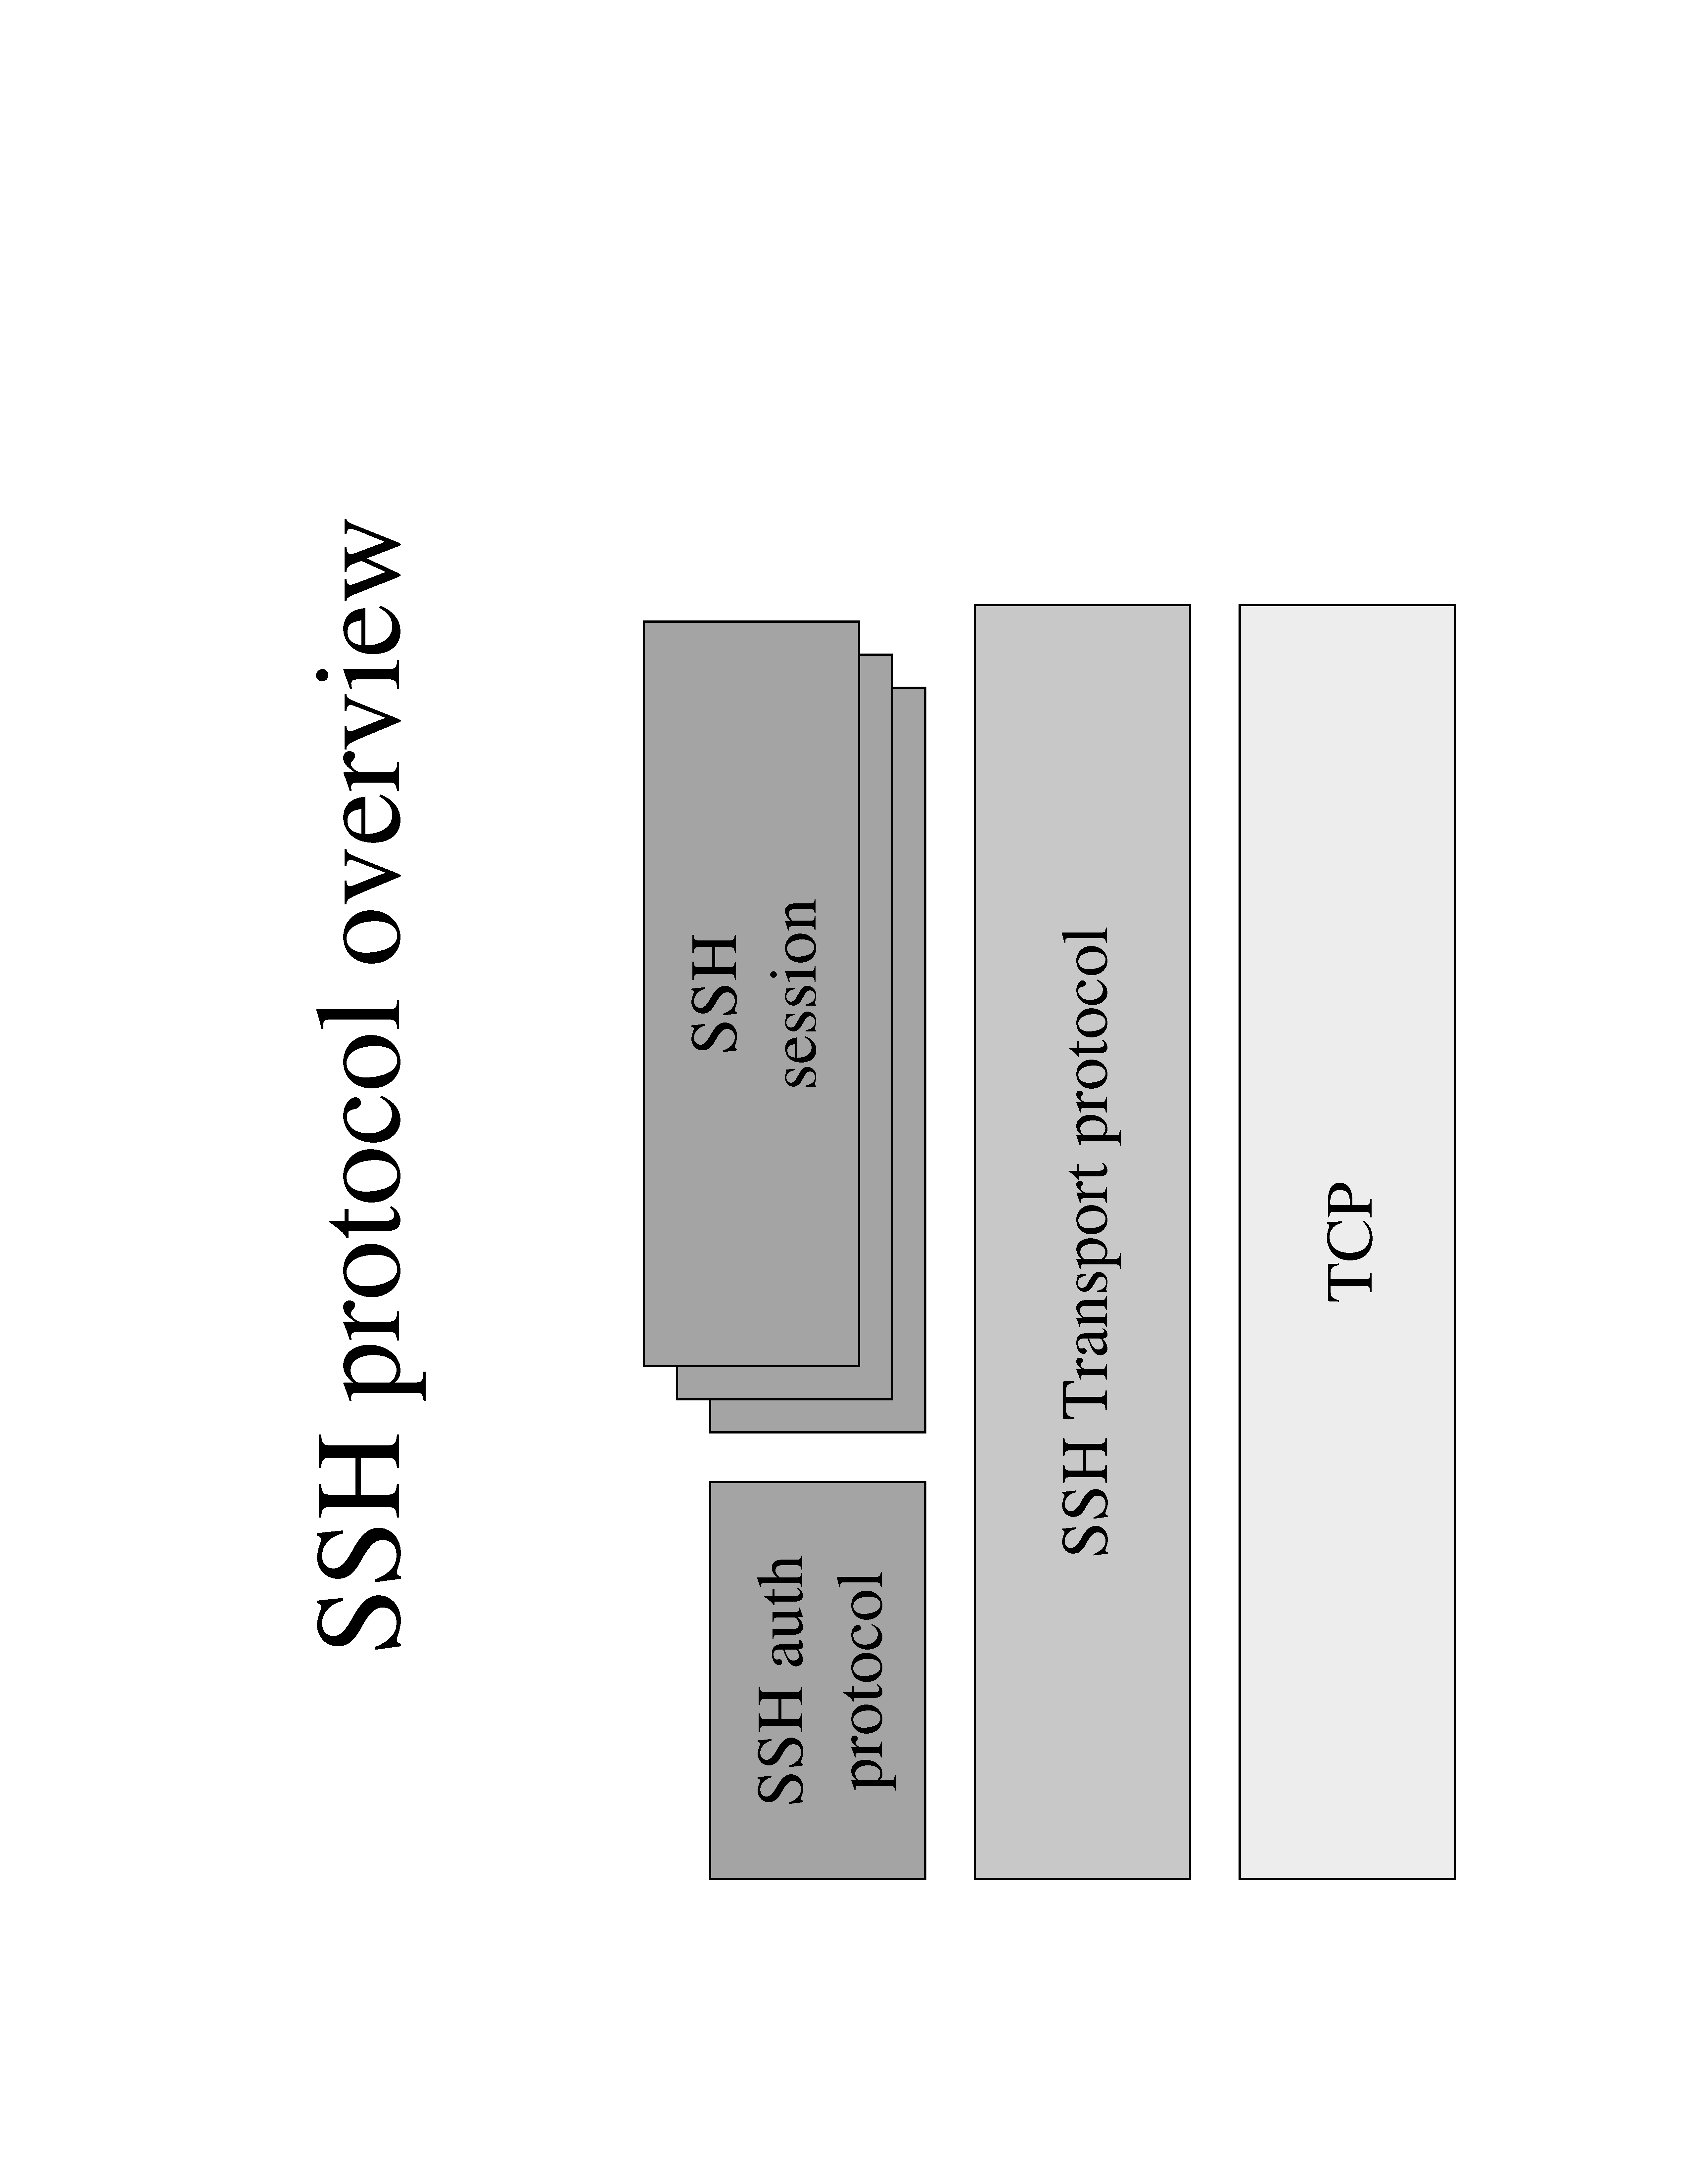
\includegraphics[clip,scale=0.4,angle=270]{ssh_overview}

\caption{\label{fig:ssh-overview} protocol hierarchy}

\end{figure}



\subsubsection{Session Initialization}

The initial handshake provides the client and server with an
opportunity to \textit{1)} perform a key exchange, \textit{(2)}
validate the server key, and \textit{(3)} negotiate an initial set of
cryptographic algorithms that will be used for the session (e.g. for
cipher, HMAC). An overview of the handshake messages are shown in
\ref{fig:ssh-init}. The steps of the protocol are as follows.  Refer
to Figure \ref{fig:ssh2-init} for details.
\begin{enumerate}
\item The SSH server sends a string of the form
  {}``SSH-2.0-\emph{software}''.  The \emph{software} string
  identifies the particular client or server.  (as a variation, it may
  also send SSH-1.99-\emph{software''} to indicate protocol version 1
  compatibility) For example, the OpenSSH 4.5 software sends
  {}``SSH-1.99-OpenSSH\_4.5''. If the client does not understand the
  protocol version, it disconnects, otherwise it sends a similar
  string to the server. After these strings are sent, all traffic uses
  the binary packet protocol shown in Figure \ref{fig:ssh-packet}.\\
%
\begin{figure}
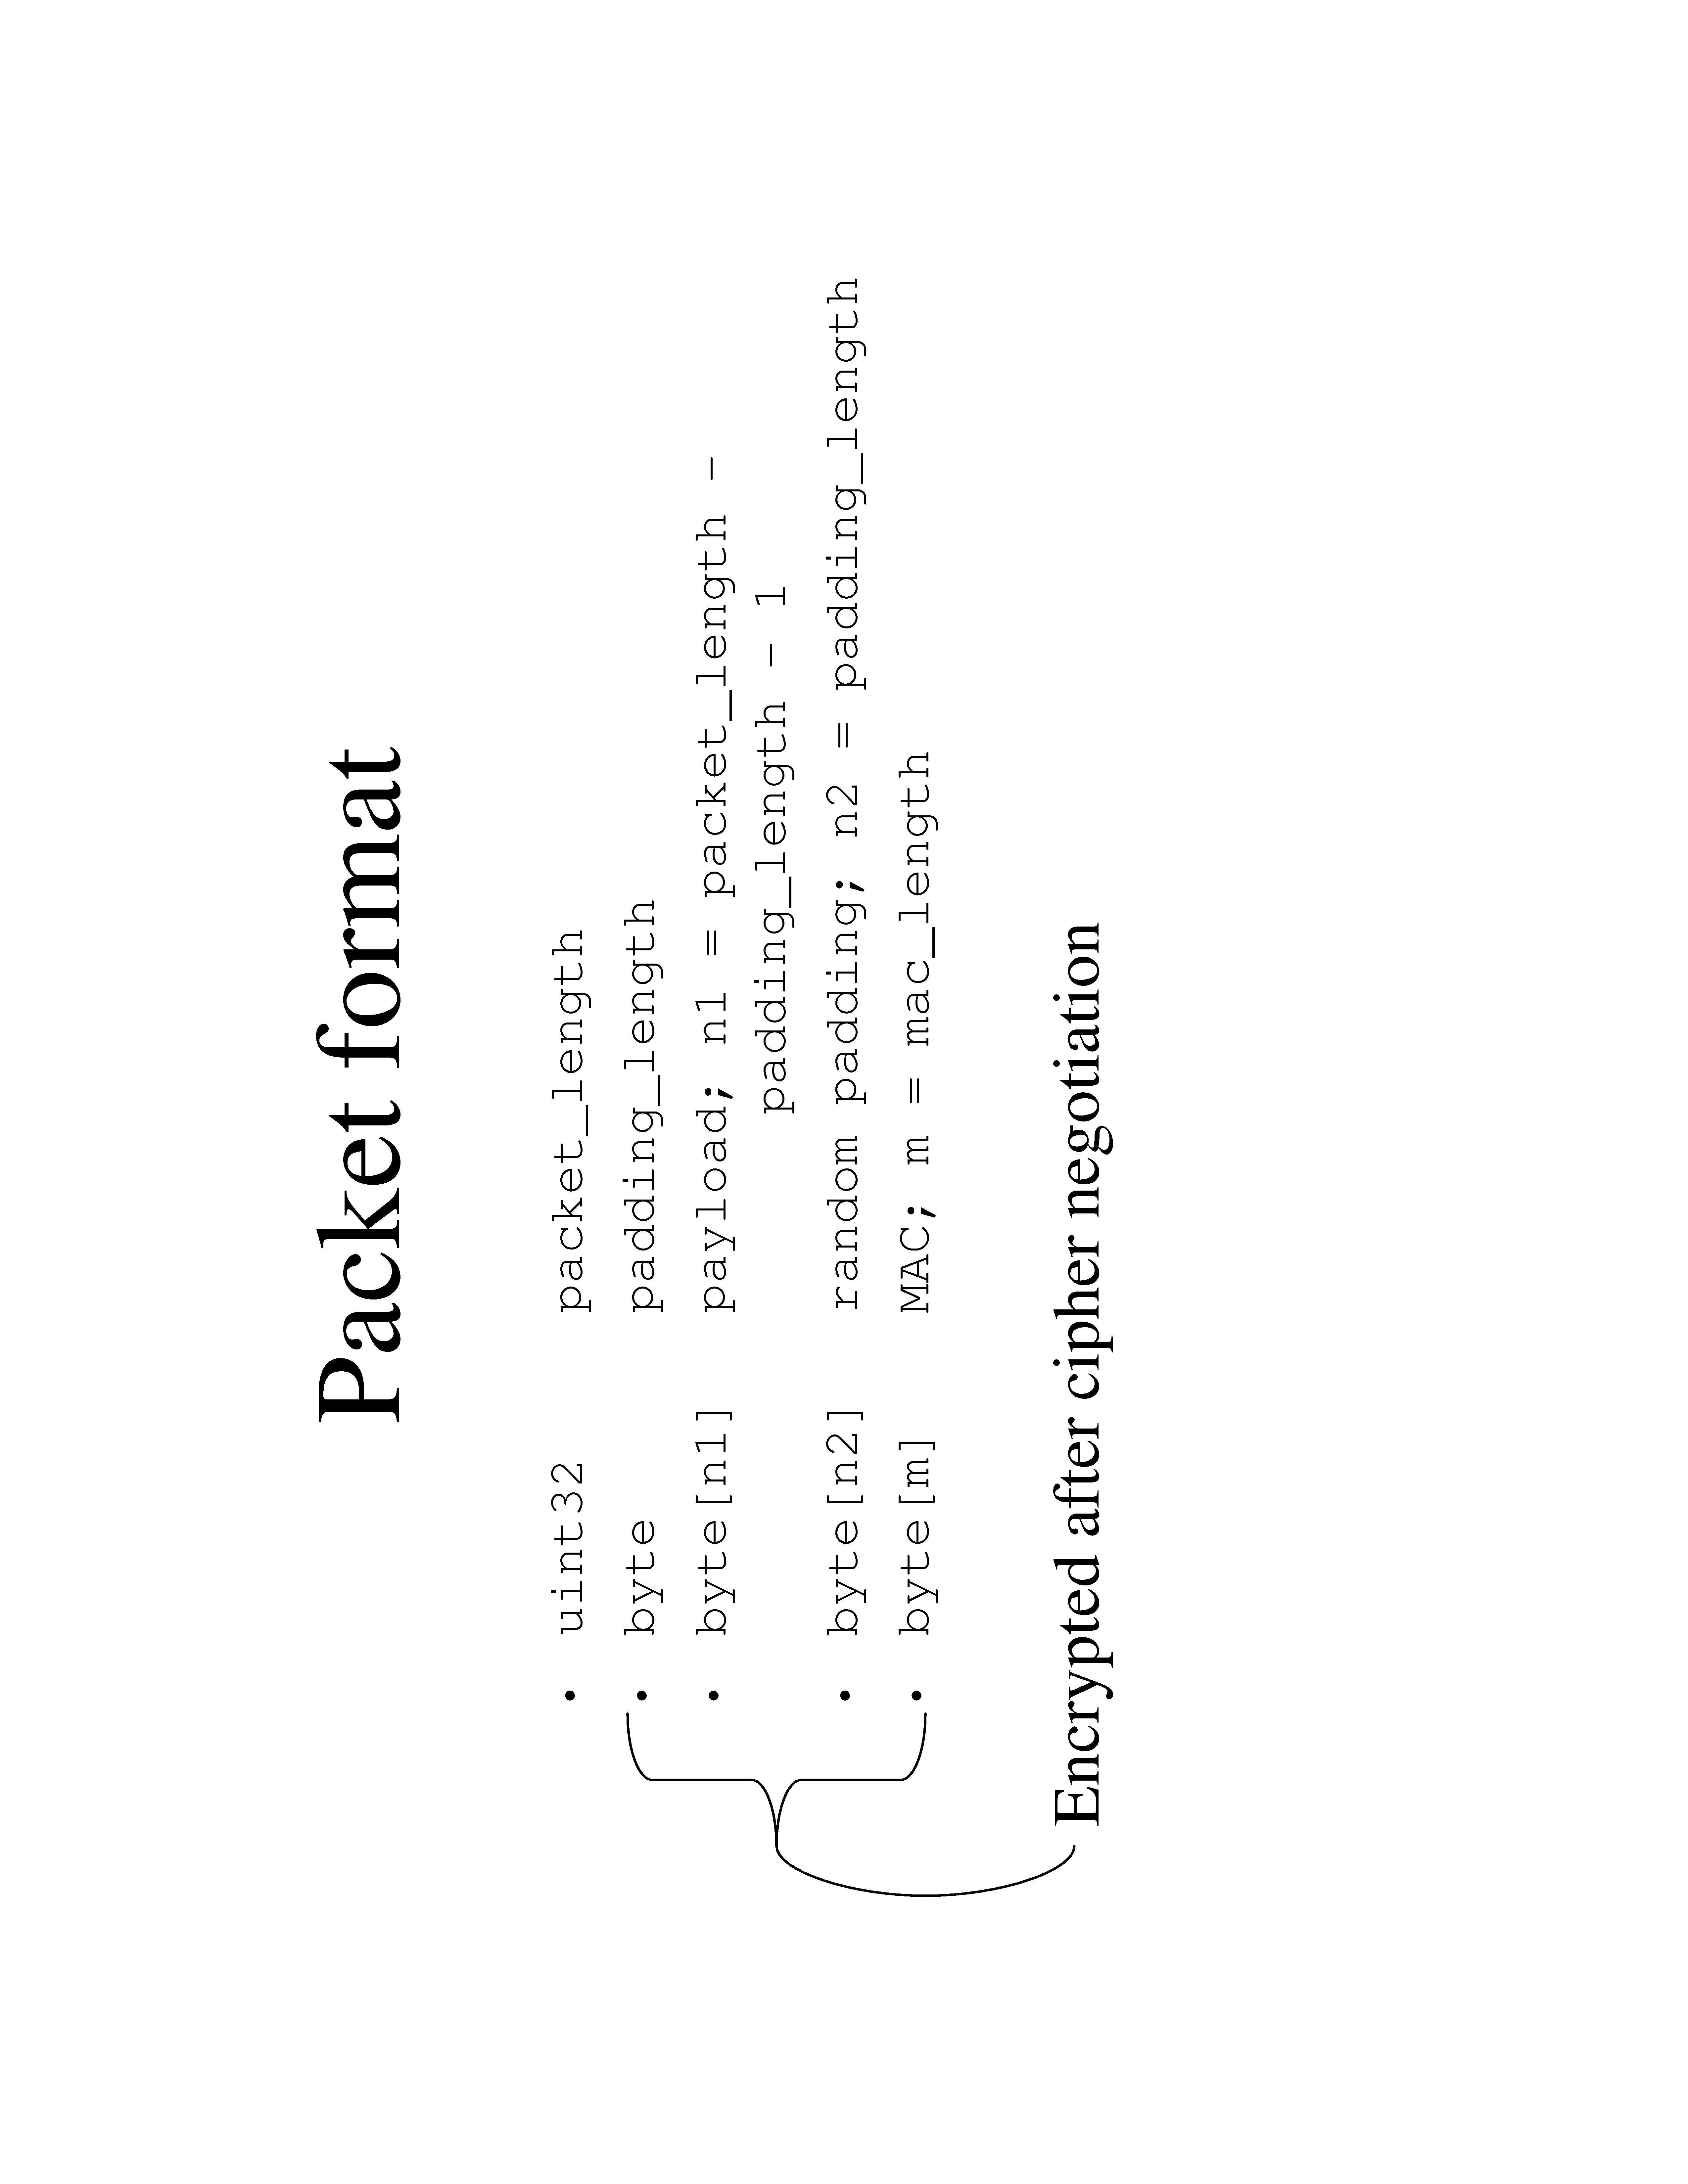
\includegraphics[clip,scale=0.4,angle=270]{ssh_packet}

\caption{\label{fig:ssh-packet} binary packet structure}

\end{figure}

\item Each party sends an SSH\_MSG\_KEXINIT message to begin the key exchange.
This message includes a list of supported ciphers, HMAC algorithms,
compression algorithms, and key exchange algorithms, ranked by preference.
For each algorithm, the parties choose the highest preference algorithm
of the client, which is also supported by the server. If one of the
algorithm lists has no algorithm in common, the connection is terminated.
%% The format of the SSH\_MSG\_KEXINIT message are as follows:

%% \begin{lyxcode}
%% ~~~~~~byte~~~~~~~~~SSH\_MSG\_KEXINIT

%% ~~~~~~byte{[}16{]}~~~~~cookie~(random~bytes)

%% ~~~~~~name-list~~~~kex\_algorithms

%% ~~~~~~name-list~~~~server\_host\_key\_algorithms

%% ~~~~~~name-list~~~~encryption\_algorithms\_client\_to\_server

%% ~~~~~~name-list~~~~encryption\_algorithms\_server\_to\_client

%% ~~~~~~name-list~~~~mac\_algorithms\_client\_to\_server

%% ~~~~~~name-list~~~~mac\_algorithms\_server\_to\_client

%% ~~~~~~name-list~~~~compression\_algorithms\_client\_to\_server

%% ~~~~~~name-list~~~~compression\_algorithms\_server\_to\_client

%% ~~~~~~name-list~~~~languages\_client\_to\_server

%% ~~~~~~name-list~~~~languages\_server\_to\_client

%% ~~~~~~boolean~~~~~~first\_kex\_packet\_follows

%% ~~~~~~uint32~~~~~~~0~(reserved~for~future~extension)
%% \end{lyxcode}
%
\begin{figure}
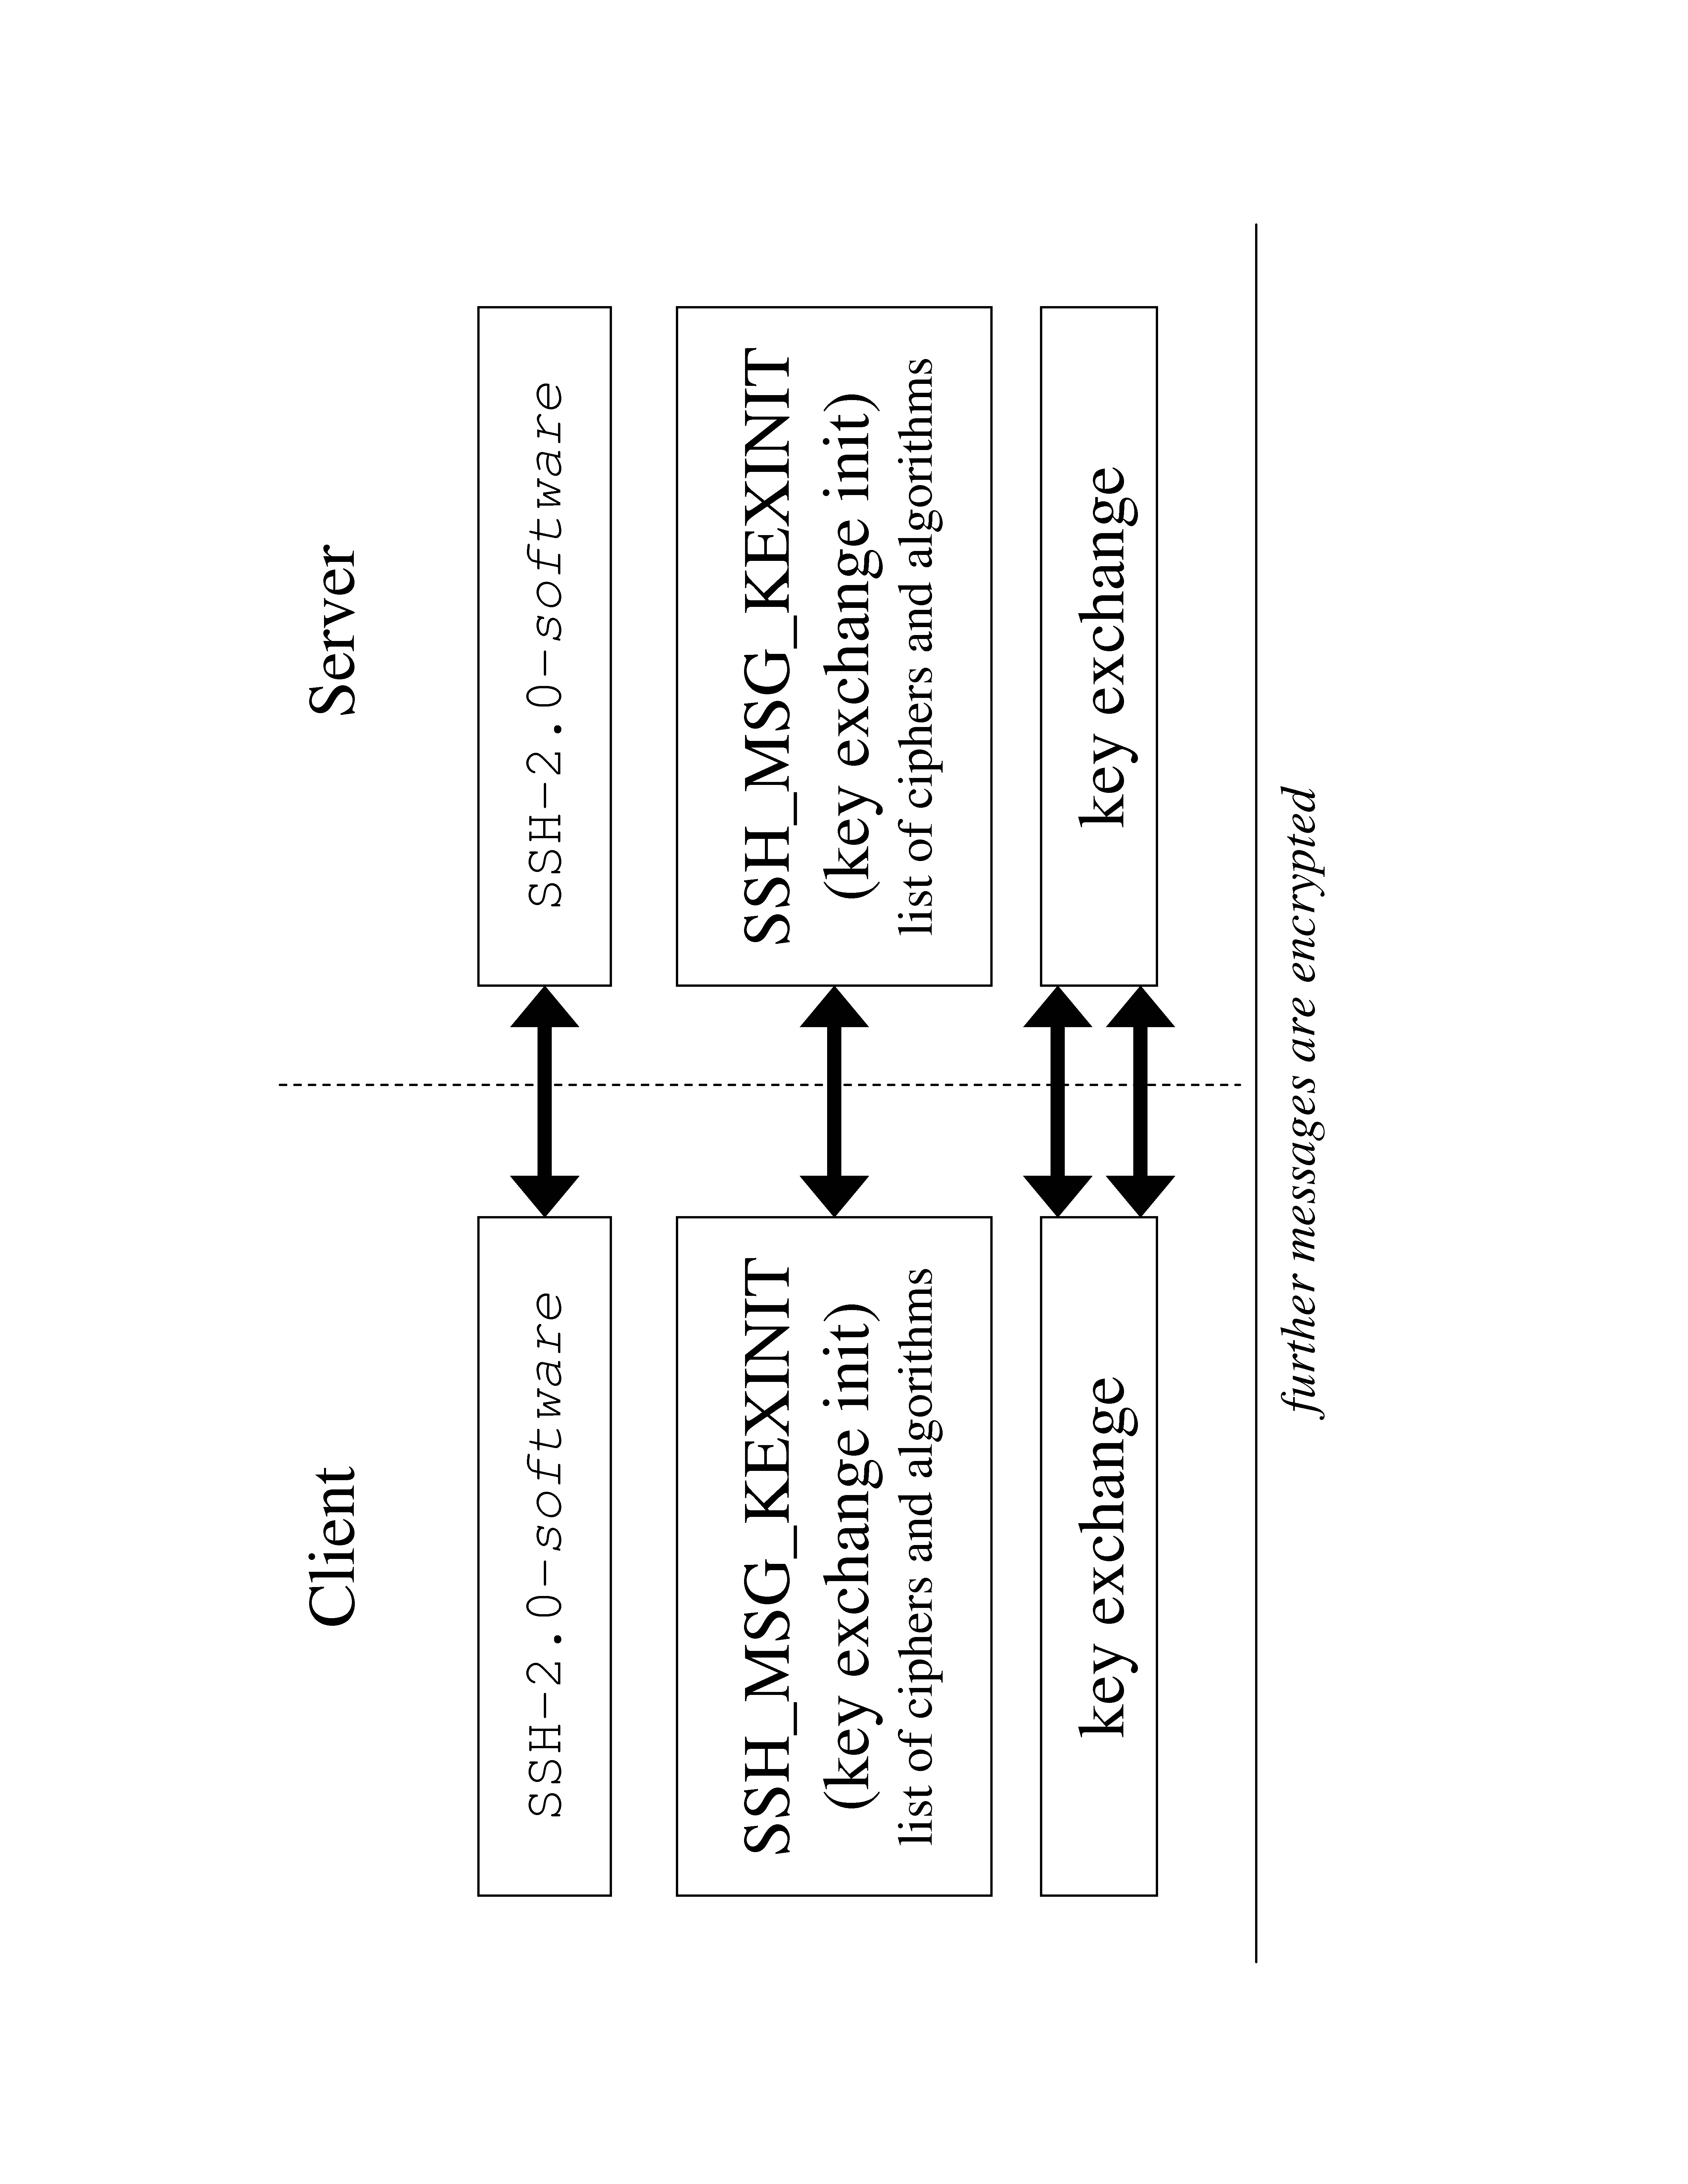
\includegraphics[clip,scale=0.4,angle=270]{ssh_init}

\caption{\label{fig:ssh-init} connection handshake protocol}

\end{figure}


%
\begin{figure}[t]
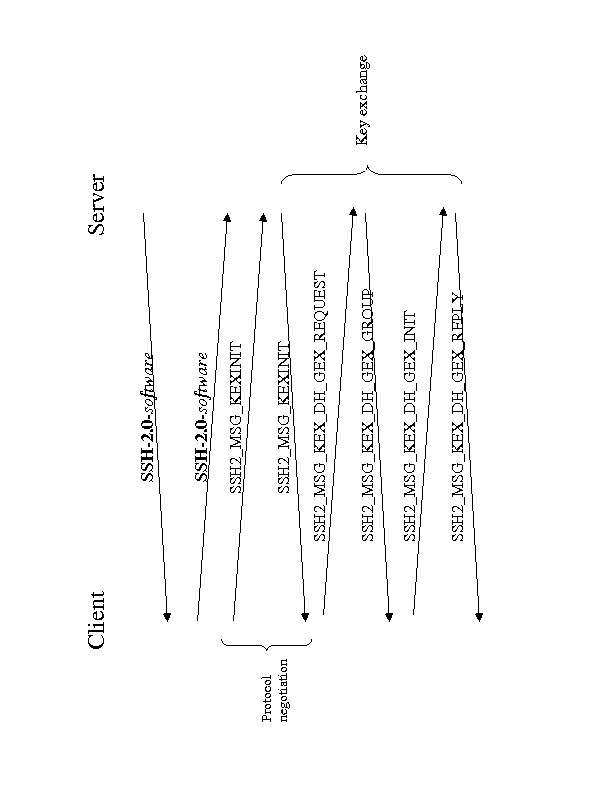
\includegraphics[clip,scale=0.4,angle=270]{ssh2_p1}

\caption{\label{fig:ssh2-init} connection handshake protocol}

\end{figure}


\item Following the handshake, the key exchange protocol is performed. The
specific algorithm used to do the key exchange is negotiated in the
previous step. The original SSH2 specification included a single Diffie-Hellman
group defined in \cite{rfc4253}. A newer and more flexible key exchange
algorithm is defined in \cite{rfc4419}. The details of key exchange
will not be discussed further. After the key exchange is complete,
all of the data in the SSH stream is encrypted using the negotiated
cipher and key. Specifically, the sequence of packets, excluding the
packet size header, shown in \ref{fig:ssh-packet} is a single stream
of plaintext encrypted by the cipher.
\end{enumerate}
At this point, the protocol handshake is complete and the client may
initiate arbitrary sub-protocols of SSH. Typically, the client will
begin the client authentication protocol, as most servers require
authentication before allowing other services to be used.


\subsubsection{Client Authentication}

When the initial handshake is complete, the client has verified the
server key, if possible, but the client has not yet authenticated to
the server. The SSH auth protocol~\cite{rfc4252} can be initiated to
perform this. The auth protocol is flexible; the SSH standard
describes several commonly-used methods of authentication, such as
password and public-key, but arbitrary authentication methods can be
added. The client selects the desired method of authentication among
those supported by the server.

The messages used in password authentication are shown in
\ref{fig:ssh-auth}.  For the purposes of this discussion, we will
assume the client is using the {}``password'' authentication
method. The steps of this authentication are as follows:
\begin{enumerate}
\item The client sends the username and password to the server in an
  SSH\_MSG\_USERAUTH\_REQUEST message. 

%% The format of this message is:

%% \begin{lyxcode}
%% ~~~~~~byte~~~~~~SSH\_MSG\_USERAUTH\_REQUEST

%% ~~~~~~string~~~~user~name~in~ISO-10646~UTF-8~encoding~{[}RFC3629{]}

%% ~~~~~~string~~~~\textquotedbl{}password\textquotedbl{}

%% ~~~~~~boolean~~~FALSE

%% ~~~~~~string~~~~plaintext~password~in~ISO-10646~UTF-8~encoding~


%% \end{lyxcode}
\item If the server does not support the {}``password'' method chosen,
or the password is incorrect, the server will respond with an SSH\_MSG\_USERAUTH\_FAILURE
message. If the password is correct, the server sends a SSH\_MSG\_USERAUTH\_SUCCESS
message, and the client may begin requesting services. (The server
may also send a SSH\_MSG\_USERAUTH\_BANNER packet to communicate information
directly to the user. It is analogous to the /etc/issue file used
in standard Unix systems to display a message at a login prompt)
\end{enumerate}
%
\begin{figure}
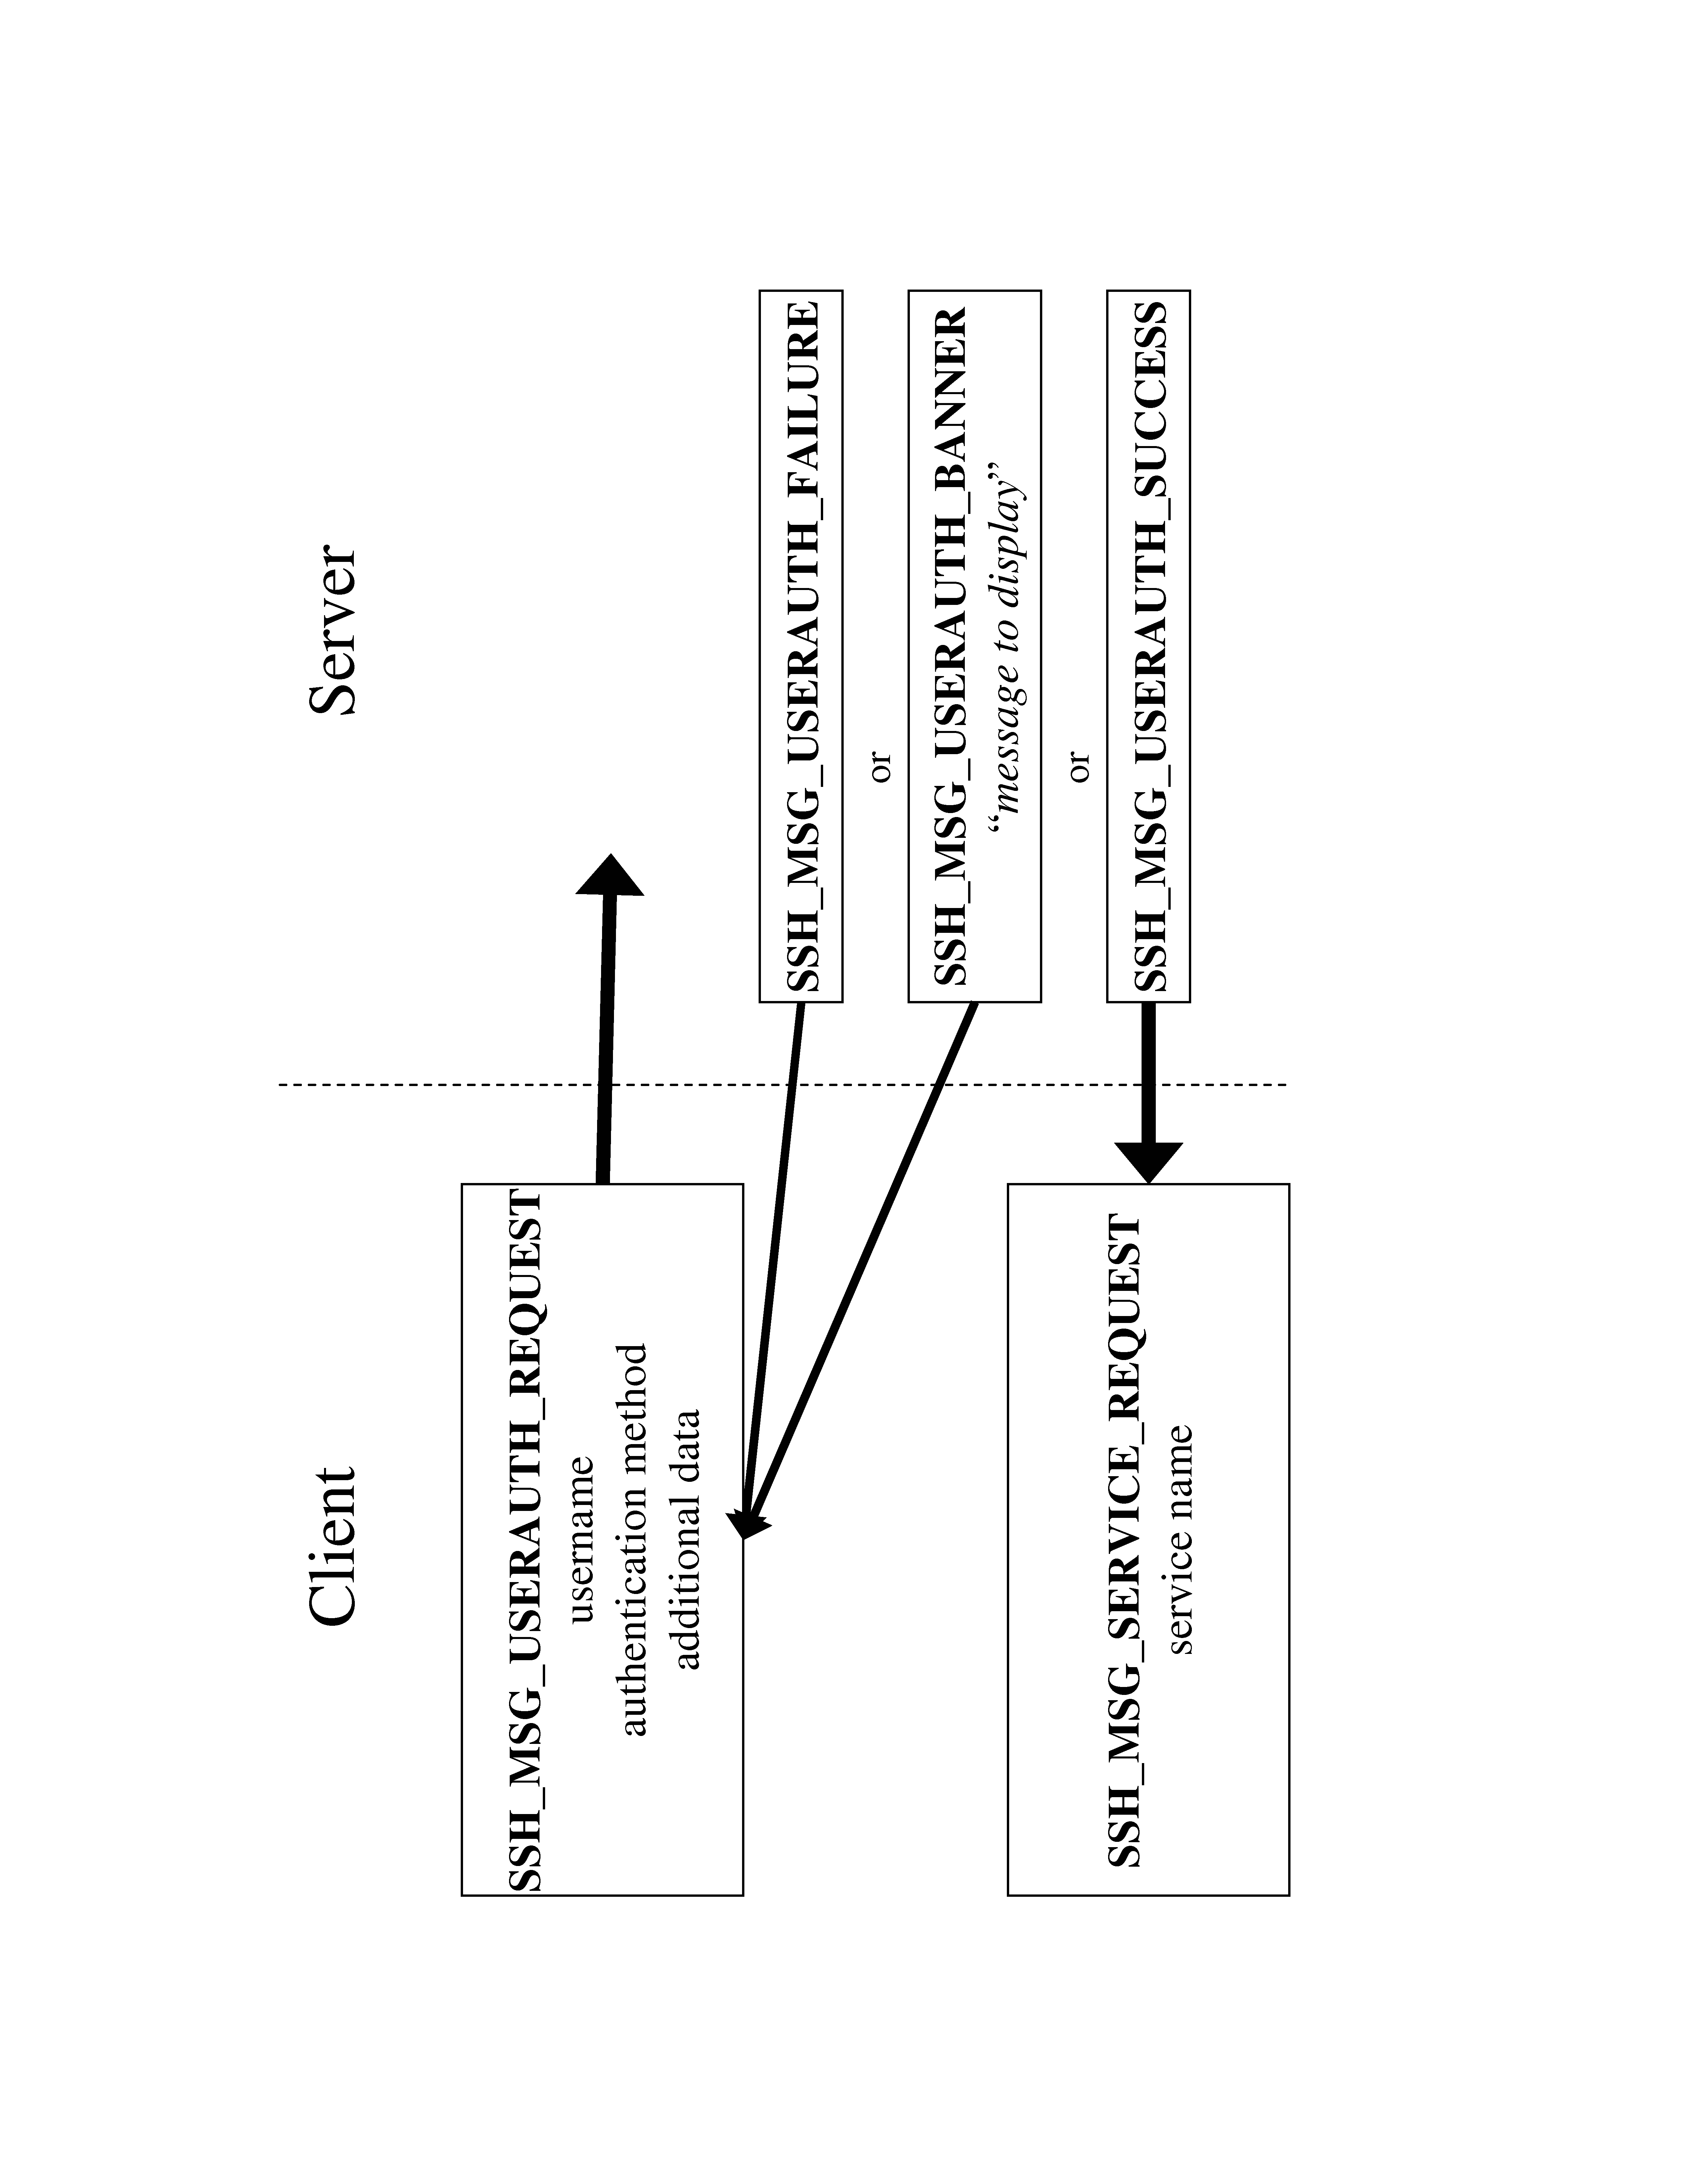
\includegraphics[clip,scale=0.4,angle=270]{ssh_auth}

\caption{\label{fig:ssh-auth} authentication protocol messages}

\end{figure}


The password is sent directly from the client to the server in a
packet. Thus, the only protection from eavesdroppers is the encryption
applied at the SSH transport layer. There is no protection of the
client's authentication credentials from the server itself, so if the
server is malicious or has been compromised, an attacker will learn
everything the client sends, and can potentially impersonate the
client at another time.


\subsection{Man in the Middle Attack}

As mentioned in the overview, as well as the previous section, the SSH
protocol is vulnerable to password compromise. An attacker can exploit
the insecurity of password transmission by mounting a \emph{man in the
  middle} (MITM) attack. Although the protocol does provide some
protection against MITM in the form of host key authentication, there
are several ways in which an attacker can thrwart this protection:
\begin{enumerate}
\item If the attacker manages to steal the host key, then the attacker can
successfully impersonate the server without detection. There is no
other means for the client to authenticate the server.
\item If the client does not know the server's host key, then the host
  cannot be authenticated unless the client has an alternative trusted
  channel to validate the host key. As mentioned in the overview, the
  following message is typically displayed by the OpenSSH client when
  connecting to a server with an unknown key\\
%
\begin{minipage}[t]{1\columnwidth}%
\begin{lyxcode}


The~authenticity~of~host~'server~(1.2.3.4)'~can't~be~established.

RSA~key~fingerprint~is~3f:76:22:43:c2:03:b9:71:b0:31:ce:87:37:45:cb:02.~

Are~you~sure~you~want~to~continue~connecting~(yes/no)?
\end{lyxcode}
%
\end{minipage}\\

Practically speaking, it may be inconvenient for a user to authenticate
the server using this message and make a correct decision. It is easy
to imagine a user simply answering yes in order to bypass the inconvenience. 
\item Even if the client does know the server's key, the there is no
  guarantee that a user would refuse to connect even if the
  authentication fails. In fact, there are several reasonable
  explanations for why a user may choose to accept a failed
  authentication and continue with the connection. For example, the
  user might think the server key changed for a non-malicious reason
  such as an operating system upgrade where the administrator forgot
  to backup the old key.
\end{enumerate}

While the only method that guarantees the success of the attacker is
\textit{(1)}, each poses a real security problem for users of SSH.

\subsection{SPAKA using SFE}

As previously hinted, this vulnerability can be mitigated by using
additional secrets which are shared between the client and server. The
password is a convenient shared secret already in common use
today. Typically, a password is considered only as a means of
authenticating a client to a server, but with certain protocols a
password can also be used for simultaneous mutual authentication in a
way that is secure, and does not compromise the password if the server
is malicious. Such protocols are known as \emph{secure password and
  key authentication} (SPAKA).

It is important to note that a {}``password'' need not be a constant
string that the user remembers over a long period of time, it can be
any string that serves as a mutual authenticator. For example, secure
ID tokens that display constantly changing strings, time synchronized
with the server, are considered to be a more secure alternative to
traditional passwords, such alternatives are readily usable in SPAKA
protocols.

The design of previous SPAKA protocols~\cite{brainard03} suggests that
SFE can be applied generally to the SPAKA problem. Here is a general
SPAKA construction based on SFE:

\begin{enumerate}

\item Let $X$ be the user's password, $Y=H(X)$ be a hash of $X$.

\item Let $C$ be the client and $S$ be the server. $C$ and $S$ participate
in a secure evaluation of the following function $f$, where $C$
provides input $X$ and $S$ provides input $Y$. $C$ and $S$ both
receive the same output from $f$, which is a single bit denoting a
boolean value.
\[
f(X,Y)=_{def} \left(Y=H\left(X\right)\right)
\]
If the value of the $f$ is $false$ then it is evident that one of the
parties did not possess the shared secret, and the mutual
authentication fails. Otherwise the mutual authentication succeeds.

\end{enumerate}

Notice that $f$ is nothing more than a variant of the well-known
millionaire problem, where the relational predicate used is equality
rather than less than or greater than. If $f$ is evaluated securely,
then $C$ and $S$ are guaranteed not to learn any information about the
computation except for the single bit of output, thus allowing them
mutual authentication without revealing any information to potential
attackers. This authentication scheme can be integrated into
implementations of the SSH protocol trivially to provide protection
from the MITM attack previously described.

%
\begin{comment}
\begin{enumerate}
\item Practical SSH paper
\item New protocol paper
\item Theoretical paper
\item Graduate!!!
\end{enumerate}

\end{comment}
{}


\section{Implementation}

We implemented an SSH client and server that incorporate this SPAKA
protocol. The following components were used:
\begin{enumerate}
\item The Dropbear SSH client and server. We chose to use this client
because of it's small and simple codebase.
\item The SFE-Tools secure function evaluation compiler first described
by Kruger \textit{et al.}
\end{enumerate}
A new authentication method was defined in the client and server code
using the extensible SSH architecture. To initiate the SPAKA
authentication protocol, the client sends an authorization protocol
request:
\begin{lyxcode}
~~~~~~byte~~~~~~SSH\_MSG\_USERAUTH\_REQUEST

~~~~~~string~~~~username

~~~~~~string~~~~\textquotedbl{}sfeauth\textquotedbl{}

~~~~~~boolean~~~FALSE
\end{lyxcode}
The server responds with the type of password hashing used to store
passwords on this system. Examples include {}``DES'' for the traditional
UNIX password crypt function, and {}``MD5'' for the default password
hashing algorithm used on most modern Linux systems. 
\begin{lyxcode}
~~~~~~byte~~~~~~SSH\_MSG\_USERAUTH\_RESPONSE

~~~~~~string~~~~username

~~~~~~string~~~~\textquotedbl{}MD5\textquotedbl{}

~~~~~~boolean~~~FALSE
\end{lyxcode}
After this exchange, the client prepares an encrypted circuit corresponding
to the hashing method in use. The underlying SFE protocol runs, wrapped
inside SSH messages SSH\_MSG\_USERAUTH\_MSG1 and SSH\_MSG\_USERAUTH\_MSG2.

\section{Related Work}

\subsection{SPAKA}

\emph{Secure Password and Key Authentication} (SPAKA) is a class of
authentication protocols first described in \cite{bellovin92}. SPAKA
protocols are designed to guarentee confidentiality of secrets even
against active adversaries. There have been various SPAKA protocols
proposed in the literature with varying properties. A recent SPAKA
protocol is presented in \cite{brainard03}. In this protocol, the
user's password $P$ is split into two shares: $P_{1}$ and $P_{2}$.
The value of $P$ can not be derived from either of the two shares
alone, and each share is stored on a seperate server. To perform the
protocol, the client splits $P$ into different shares $P_{1}'$ and
$P_{2}'$, and sends these values to the servers. The servers then
perform an evaluation protocol to determine if $P_{1}\oplus P_{2}=P_{1}'\oplus P_{2}'$.

\bibliographystyle{plain}
\bibliography{somesh,ssh}

\end{document}
